{\bfseries МРНТИ 50.41.17}

\section{ПРИМЕНЕНИЕ ИНТЕЛЛЕКТУЛЬНЫХ СИСТЕМ ПОЖАРНОЙ БЕЗОПАСНОСТИ В УМНЫХ ГОРОДАХ}
\begin{center}
{\bfseries А.Д. Бургегулов\textsuperscript{1,2*}, Т.Ж.
Мазаков\textsuperscript{1,2}, Г.З. Зиятбекова\textsuperscript{1,2}, А.А.
Саметова\textsuperscript{2}, Б.У.Джолдасова\textsuperscript{2}}

\textsuperscript{1}Институт информационных и вычислительных технологий
КН МНВО РК, Алматы, Казахстан

\textsuperscript{2}Казахский национальный университет имени аль-Фараби,
Алматы, Казахстан,

e-mail: dizel\_kz@bk.ru
\end{center}

В статье обсуждаются различные аспекты умных систем пожарной
безопасности в умных городах. Статья рассматривает различные системы
пожаротушения, системы управления пожаром на основе IoT-технологий, а
также системы оповещения и эвакуации граждан. В данной статье были
рассмотрены преимущества и недостатки каждой системы, а также примеры их
реализации в реальных умных городах. Обсуждение применимости умных
технологий в разных городских условиях и приведено сравнение различных
систем пожарной безопасности. В заключении были представлены перспективы
развития умных систем пожарной безопасности в будущем.

{\bfseries Ключевые слова:} IoT-технология, умный город, пожарная
безопасность, искусственный интеллект, контроллер, микропроцессорная
система, датчики температуры и давления.

\begin{center}
{\large\bfseries АҚЫЛДЫ ҚАЛАЛАРДА ИНТЕЛЛЕКТУАЛДЫ ӨРТ ҚАУІПСІЗДІГІ ЖҮЙЕЛЕРІН
ҚОЛДАНУ}

{\bfseries А.Д. Бургегулов\textsuperscript{1,2*}, Т.Ж.
Мазаков\textsuperscript{1,2}, Г.З. Зиятбекова\textsuperscript{1,2}, А.А.
Саметова\textsuperscript{2}, Б.У. Джолдасова\textsuperscript{2}}

\textsuperscript{1}Қазақстан Республикасы Ғылым және жоғары білім
министрлігі Ақпараттық және есептеуіш технологиялар институты, Алматы,
Қазақстан,

\textsuperscript{2}әл-Фараби атындағы Қазақ ұлттық университеті, Алматы,
Қазақстан,

e-mail: dizel\_kz@bk.ru
\end{center}

Мақалада ақылды қалалардағы өрт қауіпсіздігінің ақылды
жүйелерінің әртүрлі аспектілері талқыланады. Мақалада әртүрлі өрт
сөндіру жүйелері, IoT технологияларына негізделген өртті басқару
жүйелері, сондай-ақ азаматтарға алдын ала қауіптің болатынын ескерту
және эвакуациялау жүйелері қарастырылған. Бұл мақалада әр жүйенің
артықшылықтары мен кемшіліктері, сондай-ақ оларды нақты ақылды қалаларда
жүзеге асыру мысалдары қарастырылды. Әр түрлі қалалық жағдайларда ақылды
технологиялардың қолданылуын талқылау және әр алуан өрт қауіпсіздігі
жүйелерін салыстыру жайында айтылады. Қорытындыда болашақта өрт
қауіпсіздігінің ақылды жүйелерін дамыту перспективалары
ұсынылды.

{\bfseries Түйін сөздер:} IoT технологиясы,
ақылды қала, өрт қауіпсіздігі, жасанды интеллект, контроллер,
микропроцессорлық жүйе, температура мен қысым
датчиктері.

\begin{center}
{\large\bfseries APPLICATION OF INTELLIGENT FIRE SAFETY SYSTEMS IN SMART CITIES}

{\bfseries A.D. Burgegulov\textsuperscript{1,2*}, T.Zh.
Mazakov\textsuperscript{1,2}, G.Z. Ziyatbekova\textsuperscript{1,2},
A.A. Sametova\textsuperscript{2},}

{\bfseries B.U. Joldassova\textsuperscript{2}}

\textsuperscript{1}RSE Institute of Information and Computational
Technologies MSHE RK CS, Almaty, Kazakhstan,

\textsuperscript{2}Al-Farabi Kazakh National
University, Almaty, Kazakhstan,

e-mail: dizel\_kz@bk.ru
\end{center}

The article discusses various aspects of smart fire safety
systems in smart cities. The article examines various fire suppression
systems, fire control systems based on IoT-technologies, as well as
warning and evacuation systems for citizens. In this article, the
advantages and disadvantages of each system were discussed, as well as
examples of their implementation in real smart cities. Discusses the
applicability of smart technology in different urban environments and
provides a comparison of different fire safety systems. In conclusion,
the prospects for the development of smart fire safety systems in the
future were
presented.

{\bfseries Keywords:} IoT technology, smart
city, fire safety, artificial intelligence, controller, microprocessor
system, temperature and pressure
sensors.

\begin{multicols}{2}
{\bfseries Введение.} Растущее население городов и увеличение количества
городской инфраструктуры приводят к необходимости поиска новых способов
оптимизации использования ресурсов и улучшения качества жизни горожан.
Умные технологии стали ключевым фактором в развитии современных городов,
которые стремятся стать более эффективными, безопасными и экологически
устойчивыми.

Умные технологии представляют собой совокупность различных систем и
устройств, обеспечивающих сбор, анализ и использование данных для
автоматизации и оптимизации управления городской инфраструктурой. Эти
технологии могут включать в себя датчики, камеры, дисплеи, системы
управления и многое другое.

В сфере пожарной безопасности, умные технологии могут играть важную роль
в предотвращении пожаров, обнаружении пожаров в ранней стадии,
автоматическом подавлении пожаров и эвакуации граждан. Такие умные
системы также могут предоставлять данные для быстрого и эффективного
управления пожарами.

В целом, умные технологии предоставляют городам и горожанам множество
преимуществ, таких как повышение безопасности, улучшение управления
городской инфраструктурой, оптимизация потребления ресурсов и уменьшение
негативного воздействия на окружающую среду. Поэтому, развитие умных
технологий является важным направлением для создания умных городов в
будущем {[}1{]}.

{\bfseries Материалы и методы.} С ростом городской популяции и увеличением
количества зданий, включая многоэтажные здания, торговые центры и
склады, возрастает риск возникновения пожаров в городах. В то же время,
умные технологии, такие как системы мониторинга и контроля, датчики,
искусственный интеллект и т.д. предоставляют возможности для создания
более эффективных систем пожарной безопасности {[}2, 3{]}.

Также следует отметить, что умные города представляют собой сложную
инфраструктуру, и системы пожарной безопасности должны соответствовать
этим особенностям. В умном городе может использоваться большое
количество электроники, а также множество устройств с доступом к
интернету, которые могут быть подвержены пожарам и должны быть защищены.

Следовательно, обеспечение пожарной безопасности в умных городах
является необходимым для защиты жизни и имущества горожан, а также для
обеспечения устойчивого развития городской инфраструктуры {[}4-6{]}.

{\bfseries \emph{Цель и задачи исследования}}

Рассмотрим некоторые примеры существующих умных систем детектирования
пожаров, а также их преимуществ и недостатки.

Система детектирования пожаров по видеонаблюдению. Эта система
использует камеры видеонаблюдения, которые способны обнаруживать
определенные признаки пожара, такие как дым, огонь и т.д. Кроме того,
система использует алгоритмы искусственного интеллекта для обработки
видеоизображения и обнаружения пожара. Например, такую систему
используют в Техасе (США) в магазинах Walmart.

Преимущества:

\begin{enumerate}
\def\labelenumi{\arabic{enumi}.}
\item
  Система может обнаруживать признаки пожара, которые не могут быть
  обнаружены другими системами детектирования, например, огонь или дым
  на видеоизображении;
\item
  Возможно использование алгоритмов искусственного интеллекта, что
  повышает точность определения пожара;
\item
  Система может использоваться для мониторинга больших территорий,
  например, в торговых центрах или на промышленных объектах.
\end{enumerate}

Недостатки:

\begin{enumerate}
\def\labelenumi{\arabic{enumi}.}
\item
  Система может не обнаружить пожар, если видеоизображение заблокировано
  или недоступно;
\item
  Видеоизображение может содержать ложные срабатывания, если на нем есть
  элементы, похожие на признаки пожара, например, свет, солнечные лучи и
  т.д.
\item
  Требуется большое количество камер для обеспечения полного покрытия
  территории, что может быть дорого.
\end{enumerate}

Система детектирования пожаров по звуку. Эта система использует
микрофоны, чтобы обнаруживать звуки, связанные с пожаром, например,
треск огня или раскаты грома. Система также может использовать алгоритмы
искусственного интеллекта для обработки звуковых данных и определения
возможного пожара. Например, такую систему применяют в аэропорту Шанхая
(Китай).

Преимущества:

\begin{enumerate}
\def\labelenumi{\arabic{enumi}.}
\item
  Система может использоваться для мониторинга больших территорий,
  например, в аэропортах или на железнодорожных станциях.
\item
  Возможно использование алгоритмов искусственного интеллекта для
  улучшения точности обнаружения;
\item
  Система может обнаружить пожар, даже если видеоизображение недоступно
  или заблокировано.
\end{enumerate}

Недостатки:

\begin{enumerate}
\def\labelenumi{\arabic{enumi}.}
\item
  Датчики микрофонов могут быть недоступны в некоторых зонах, например,
  в помещениях со слишком высоким уровнем шума.
\item
  Система может давать ложные срабатывания, если обнаружены звуки,
  которые не связаны с пожаром, например, шумы движущегося транспорта.
\end{enumerate}

Система детектирования пожаров по температуре. Эта система использует
датчики температуры, чтобы обнаружить повышение температуры, которое
может указывать на наличие пожара. Такие системы могут быть установлены
в крупных складах, а также в промышленных зонах. Например, такую систему
применяют в крупном складе Amazon в Британии.

Преимущества:

\begin{enumerate}
\def\labelenumi{\arabic{enumi}.}
\item
  Система может использоваться для мониторинга объектов, в которых
  необходимо обеспечить постоянный контроль температуры, например, в
  промышленности.
\item
  Система может обнаружить повышение температуры, что может указывать на
  наличие пожара.
\end{enumerate}

Недостатки:

\begin{enumerate}
\def\labelenumi{\arabic{enumi}.}
\item
  Система может не обнаружить пожар, если температура пожара
  недостаточно высока для того, чтобы сработал датчик.
\item
  Система может давать ложные срабатывания, если температура повышается
  не из-за пожара, например, из-за неисправности оборудования.
\end{enumerate}

{\bfseries Результаты и обсуждение.} Система детектирования пожаров по
давлению. Эта система использует датчики давления, чтобы обнаружить
изменения давления, которые могут указывать на наличие пожара. Такие
системы могут быть установлены в объектах с вытяжными системами, такими
как кухни и прачечные, а также в промышленных зонах. Например, такую
систему применяют в одном из крупнейших розничных сетей Walmart для
обеспечения безопасности в магазинах и складах. Эта система позволяет
быстро обнаруживать пожары и максимально быстро реагировать на них,
чтобы минимизировать ущерб для имущества и безопасность персонала. Кроме
того, система может быть подключена к другим системам безопасности,
таким как системы пожаротушения и эвакуации, чтобы обеспечить более
комплексный подход к обеспечению безопасности.

Преимущества:

\begin{enumerate}
\def\labelenumi{\arabic{enumi}.}
\item
  Система может обнаружить пожар, даже если его источник не находится в
  непосредственной близости от датчика.
\item
  Система может использоваться для мониторинга объектов, в которых есть
  вытяжные системы, такие как кухни и прачечные.
\end{enumerate}

Недостатки:

\begin{enumerate}
\def\labelenumi{\arabic{enumi}.}
\item
  Система может давать ложные срабатывания, если давление повышается не
  из-за пожара, например, из-за изменения условий вентиляции.
\item
  Датчики давления могут быть недоступны в некоторых зонах, например,
  если вытяжные системы не установлены.
\end{enumerate}

Каждая из этих систем имеет свои преимущества и недостатки, и выбор
системы зависит от конкретных потребностей и условий городской
инфраструктуры: тип объекта, бюджет, доступность и т.д. Однако все эти
умные системы детектирования пожаров позволяют более быстро и точно
обнаруживать пожары, что является критически важным для обеспечения
пожарной безопасности в умных городах. Также современные технологии
позволяют объединять различные системы и сенсоры для создания более
надежной системы пожарной безопасности в умных городах {[}2{]}.

Системы детектирования пожаров на основе температуры и давления
используются во многих умных городах по всему миру для обеспечения
безопасности горожан и защиты имущества (Рис. 1).

\begin{itemize}
\item
  Например, в городе Бостон, США, установлены датчики дыма и
  температуры, которые используются для детектирования пожаров в зданиях
  и на улицах. Эти датчики также могут передавать информацию в
  диспетчерские центры, которые быстро реагируют на возможные пожары.
\item
  В Сингапуре, где многие здания оборудованы системами умного дома,
  датчики дыма и температуры также используются для детектирования
  пожаров. Кроме того, умные системы пожарной безопасности могут быть
  интегрированы с другими системами, такими как системы эвакуации и
  пожаротушения, чтобы обеспечить максимальную эффективность и
  минимизировать ущерб.
\item
  В городе Амстердам (Нидерланды), установлены датчики температуры,
  которые могут обнаруживать повышенную температуру на улицах и в
  зданиях, что может указывать на возможный пожар. Датчики связаны с
  системой мониторинга и управления, которая позволяет быстро
  обнаруживать пожары и координировать действия службы пожарной
  безопасности.
\item
  Смарт-система пожаротушения в Дубае: Эта система включает сеть
  датчиков и камер, расположенных в зданиях, которые могут обнаруживать
  пожары и отправлять информацию на пульт управления пожарной службы,
  чтобы быстро реагировать на происшествия.
\item
  Система детектирования пожаров в Лос-Анджелесе: В Лос-Анджелесе
  введена система детектирования пожаров, которая использует анализ
  облачных данных, чтобы обнаружить пожары в ранней стадии. Эта система
  также включает в себя установленные вокруг города камеры для
  наблюдения за пожарами.
\item
  Умный город Сидней: В Сиднее была введена система детектирования
  пожаров, которая использует искусственный интеллект для анализа данных
  с датчиков, которые мониторят температуру, дым, уровень кислорода и
  другие параметры. Эта система также может автоматически управлять
  системами пожаротушения, чтобы быстро предотвратить распространение
  пожара.
\end{itemize}
\end{multicols}

\begin{figure}[H]
  \centering
  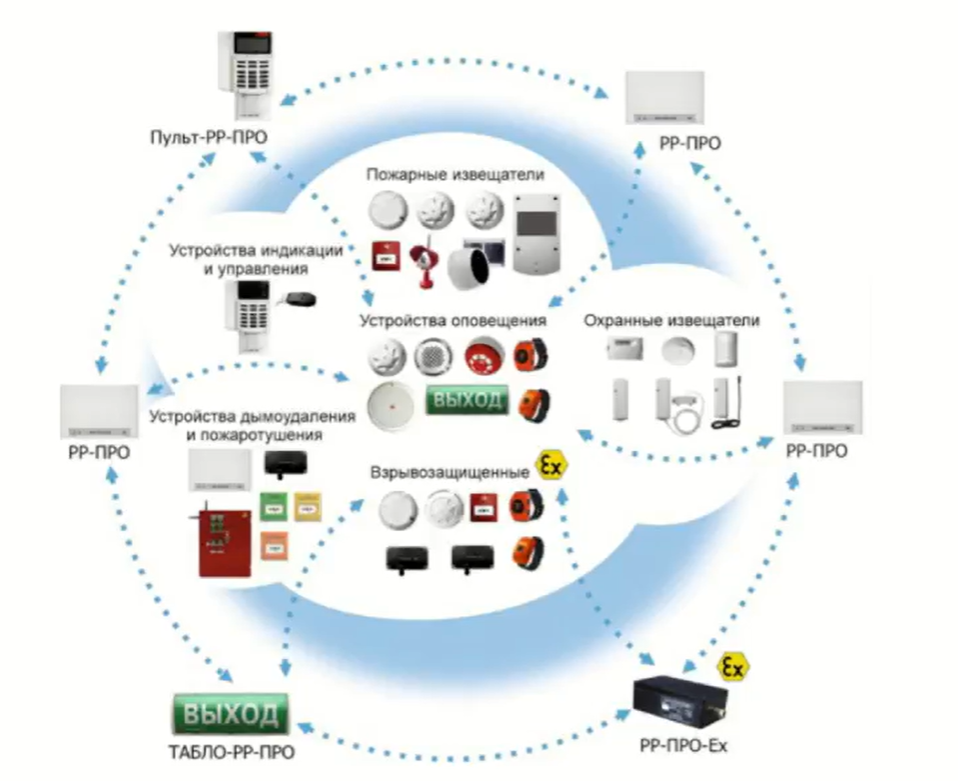
\includegraphics[width=0.8\textwidth]{image1}
  \caption{Беспроводная система пожарной сигнализации и автоматики,
  включающая в себя облачный сервис для технологического мониторинга
  {[}7{]}}
\end{figure}

\begin{multicols}{2}
В целом, умные системы детектирования пожаров имеют огромный потенциал
для обеспечения безопасности в умных городах. Однако, важно учитывать,
что каждая система имеет свои преимущества и недостатки, и выбор
конкретной системы должен основываться на специфических потребностях
города и его жителей.

Существует множество различных систем автоматического подавления
пожаров, которые используются для быстрого и эффективного тушения
возгораний. Некоторые из них включают (Рис. 2):

\begin{itemize}
\item
  Системы автоматического пожаротушения на основе газов. Эти системы
  используют различные газы, такие как аргон, диоксид углерода, азот или
  инертные газы, для тушения пожара. Газы подаются в помещение через
  сеть трубопроводов и распыляются по всей площади. Газы поглощают
  тепло, замедляют химические реакции и удаляют кислород, что приводит к
  ликвидации пожара.
\item
  Системы автоматического пожаротушения на основе жидкостей. Эти системы
  используют жидкие вещества, такие как вода, пены или специальные
  жидкости, для тушения пожара. Жидкости подаются в помещение через сеть
  трубопроводов и распыляются на поверхности горящих материалов.
  Жидкости охлаждают горящие поверхности, удаляют тепло и предотвращают
  распространение пламени.
\item
  Системы автоматического пожаротушения на основе порошков. Эти системы
  используют порошки, такие как сульфат алюминия или бикарбонат натрия,
  для тушения пожара. Порошки подаются в помещение через сеть
  трубопроводов и распыляются на поверхности горящих материалов. Порошки
  задерживают кислород, замедляют химические реакции и удаляют тепло,
  что приводит к ликвидированию пожара.
\item
  Системы автоматического пожаротушения на основе пены. Эти системы
  используют пену, которая создается путем смешивания воды и
  специального раствора, для тушения пожара. Пена подаются в помещение
  через сеть трубопроводов и распыляются на поверхности горящих
  материалов. Пена уменьшает количество кислорода, снижает температуру и
  удаляет тепло, что приводит к тушению пожара.
\end{itemize}

\end{multicols}

\begin{figure}[H]
  \centering
  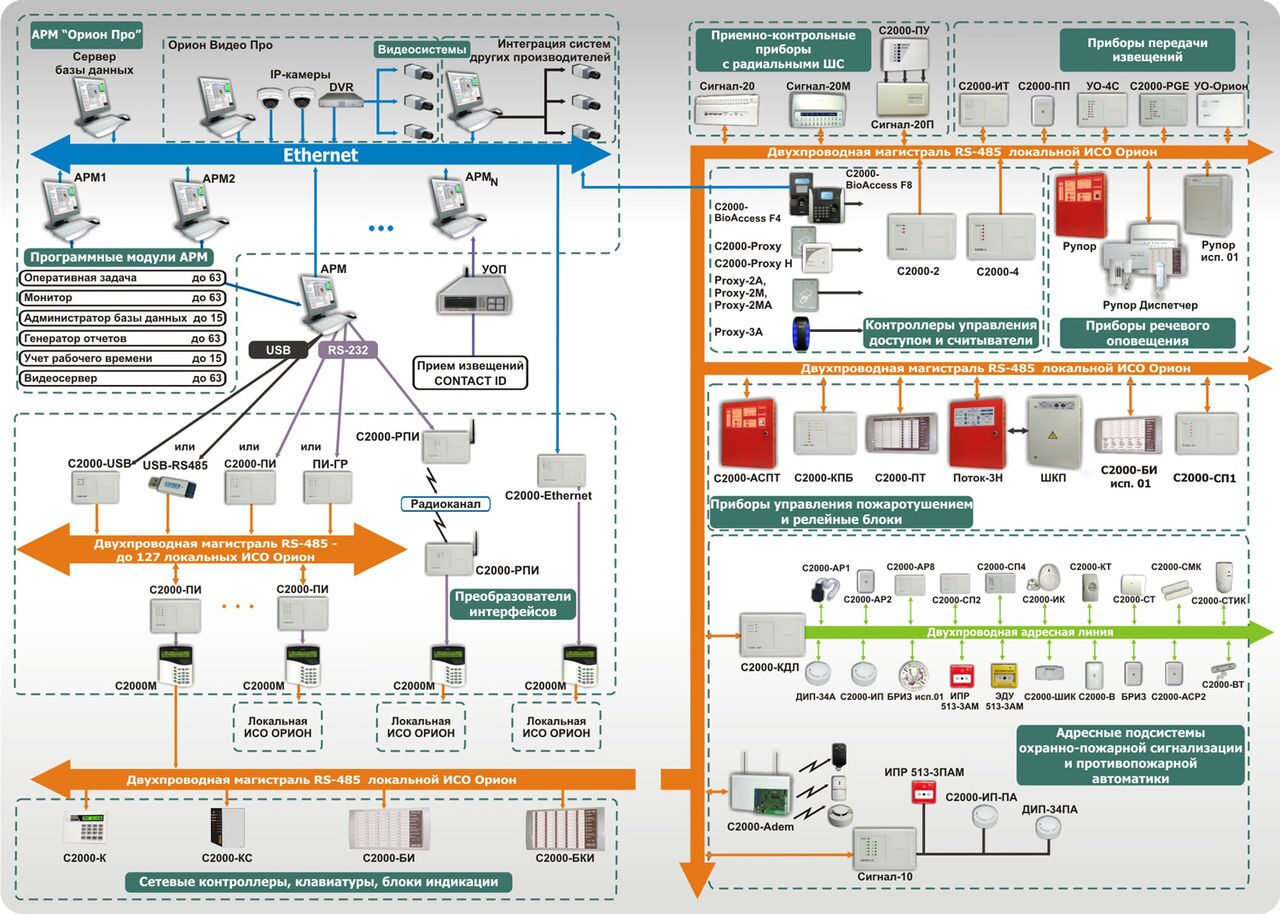
\includegraphics[width=0.8\textwidth]{image2}
  \caption{Пример построения пожарной сигнализации на основе системы BOLID,
которая включает три автоматические установки пожаротушения (порошковое,
газовое, водяное)}
\end{figure}

\begin{multicols}{2}

Каждая система автоматического подавления пожаров имеет свои
преимущества и недостатки. Ниже приведены некоторые из них:

Система автоматического пожаротушения водой:

Преимущества:

\begin{enumerate}
\def\labelenumi{\arabic{enumi}.}
\item
  Это наиболее распространенная и экономически выгодная система тушения
  пожара.
\item
  Вода доступна повсюду и является относительно дешевым ресурсом.
\item
  Она недорога в установке и обслуживании.
\item
  Система довольно проста в использовании.
\end{enumerate}

Недостатки:

\begin{enumerate}
\def\labelenumi{\arabic{enumi}.}
\item
  Вода может нанести вред имуществу, которое находится в зоне пожара.
\item
  Она неэффективна при тушении пожаров, связанных с электрооборудованием
  и маслом.
\item
  При наличии чрезмерного количества воды может возникнуть опасность
  затопления здания.
\end{enumerate}

Система автоматического пожаротушения газом:

Преимущества:

\begin{enumerate}
\def\labelenumi{\arabic{enumi}.}
\item
  Газы, такие как углекислый газ, галогенные газы и аргон, не повреждают
  имущество при тушении пожара.
\item
  Газы не оставляют следов и не оказывают негативного влияния на
  окружающую среду.
\item
  Система автоматического пожаротушения газом может быть легко
  интегрирована в существующую систему пожарной безопасности.
\end{enumerate}

Недостатки:

\begin{enumerate}
\def\labelenumi{\arabic{enumi}.}
\item
  Газы могут быть опасными для здоровья людей и животных.
\item
  Система автоматического пожаротушения газом может быть дорогой в
  установке и обслуживании.
\end{enumerate}

Система автоматического пожаротушения пеной:

Преимущества:

\begin{enumerate}
\def\labelenumi{\arabic{enumi}.}
\item
  Пена не повреждает имущество при тушении пожара.
\item
  Система автоматического пожаротушения пеной работает очень быстро и
  эффективно.
\item
  Пена обладает дополнительными свойствами охлаждения, которые могут
  помочь предотвратить повторное возгорание.
\end{enumerate}

Недостатки:

\begin{enumerate}
\def\labelenumi{\arabic{enumi}.}
\item
  Пена может вызывать коррозию электрооборудования.
\item
  Система автоматического пожаротушения пеной может быть дорогой в
  установке и обслуживании.
\end{enumerate}

Система автоматического пожаротушения порошком:

Преимущества:

\begin{enumerate}
\def\labelenumi{\arabic{enumi}.}
\item
  Порошок быстро тушит пожар, потому что быстро затушивает пламя и
  снижает температуру.
\item
  Порошковые системы довольно надежны и могут использоваться для тушения
  различных типов пожаров, включая горючие жидкости, газы и твердые
  вещества.
\item
  Порошковые системы относительно просты в использовании и обслуживании.
\end{enumerate}

Недостатки:

\begin{enumerate}
\def\labelenumi{\arabic{enumi}.}
\item
  Порошок может оставлять остатки на поверхностях, что может быть
  проблемой для некоторых промышленных процессов.
\item
  Порошковые системы не подходят для использования в областях с высокой
  влажностью, так как вода может склеивать порошок и делать его менее
  эффективным.
\item
  Порошок может быть вреден для животных и людей, поэтому следует быть
  осторожными при использовании в жилых зонах.
\end{enumerate}

Система автоматического пожаротушения углекислым газом:

Преимущества:

\begin{enumerate}
\def\labelenumi{\arabic{enumi}.}
\item
  Углекислый газ быстро тушит пожары и не оставляет остатков.
\item
  Углекислый газ не повреждает электронное оборудование и другие
  чувствительные предметы.
\item
  Системы тушения углекислым газом могут использоваться в небольших и
  крупных помещениях.
\end{enumerate}

Недостатки:

\begin{enumerate}
\def\labelenumi{\arabic{enumi}.}
\item
  Углекислый газ может быть опасен для людей, поэтому следует быть
  осторожными при использовании в жилых зонах.
\item
  Углекислый газ может быть дорогим в производстве, что может повлиять
  на стоимость системы пожаротушения.
\item
  Системы тушения углекислым газом могут потребовать дополнительных
  работ по установке и обслуживанию, что может повлиять на стоимость и
  сложность системы.
\end{enumerate}

Некоторые примеры реализации систем автоматического подавления пожаров в
умных городах:

\begin{itemize}
\item
  Шанхай, Китай: В рамках проекта по созданию умного города в Шанхае
  были установлены системы автоматического пожаротушения в некоторых
  зданиях и объектах города, включая жилые дома, торговые центры и
  склады. Системы используют различные методы тушения пожара, включая
  использование воды, газов и порошка.
\item
  Сеул, Южная Корея: В Сеуле были установлены системы автоматического
  пожаротушения в метрополитене города. Системы используют воду для
  тушения пожаров и были разработаны с учетом особенностей
  метрополитена, включая наличие высоковольтных линий и систем
  вентиляции.
\item
  Дубай, ОАЭ: В Дубае была установлена система автоматического
  пожаротушения в самом высоком здании в мире - небоскребе Burj Khalifa.
  Система использует воду для тушения пожаров и была разработана с
  учетом особенностей здания, включая его высоту и сложную архитектуру.
  Городская команда пожарных внедрила систему Fireye, которая использует
  искусственный интеллект для обнаружения возгораний и автоматического
  оповещения пожарных. Система включает в себя более 16 000 датчиков и
  позволяет реагировать на пожары мгновенно.
\item
  Город Копенгаген в Дании: в Копенгагене внедрена система пожарной
  безопасности, которая использует данные датчиков качества воздуха для
  обнаружения изменений в концентрации угарного газа и оповещения о
  пожарах.
\item
  Город Торонто в Канаде: в Торонто внедрена система пожарной
  безопасности, которая использует умные датчики, установленные на
  каждом этаже здания, для обнаружения пожаров. Датчики синхронизированы
  с центральной системой управления, которая автоматически оповещает
  пожарных и предоставляет информацию о месте возгорания.
\item
  Город Сеул в Южной Корее: в Сеуле установлены умные датчики дыма,
  которые используются для обнаружения пожаров в многоэтажных зданиях.
  Датчики сигнализируют о пожаре, а затем система автоматического
  пожаротушения, установленная на каждом этаже, начинает работу.
\item
  Барселона, Испания: В Барселоне была установлена система
  автоматического пожаротушения в здании местного музея. Система
  использует газ для тушения пожаров и была разработана с учетом
  особенностей здания, включая его историческую ценность и наличие
  хрупких экспонатов.
\end{itemize}

Умные системы управления пожаром используют сенсоры и другие технологии,
чтобы обнаруживать пожары и принимать соответствующие меры для их
тушения. Они могут включать в себя следующие компоненты (Рис. 3):

\begin{itemize}
\item
  Системы управления пожаротушением: эти системы используют различные
  технологии, такие как датчики дыма и тепла, чтобы обнаруживать пожары
  и автоматически активировать системы пожаротушения, такие как системы
  дренажных шлангов и автоматические установки пожаротушения.
\item
  Системы управления дверьми: эти системы используются для контроля
  доступа и предотвращения распространения огня через двери. Они могут
  быть программируемыми для автоматического закрытия и блокировки
  дверей, если возникает пожар.
\item
  Системы управления эвакуацией: эти системы предназначены для быстрой и
  эффективной эвакуации людей из здания в случае пожара. Они могут
  включать в себя автоматические оповещения и инструкции для эвакуации,
  системы связи и навигации, а также интегрированные системы контроля
  доступа для предотвращения паники и хаоса.
\item
  Системы мониторинга окружающей среды: эти системы используют сенсоры
  для наблюдения за уровнем кислорода, угарного газа и других вредных
  веществ в окружающей среде. Они также могут контролировать температуру
  и влажность, чтобы определить риски возгорания.
\end{itemize}

\begin{center}
  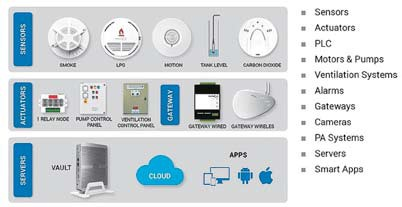
\includegraphics[width=\linewidth]{image3}
  \captionof{figure}{Элементы системы пожарной безопасности на основе IoT}
\end{center}

Примеры умных систем управления пожаром включают в себя систему
«СМАРТ-ПОЖАР» в Москве, которая включает в себя датчики дыма, тепла и
газа, а также систему оповещения и навигации для эвакуации людей.

Еще один пример - система управления пожаром в торговом центре «Cityon
Xi\textquotesingle an» в Китае, которая включает в себя системы
мониторинга окружающей среды, автоматические установки пожаротушения и
систему управления дверьми для предотвращения распространения огня.

Ниже приведены преимущества и недостатки нескольких типов умных систем
управления пожаром:

Системы управления пожаром на основе облака данных.

Преимущества:

\begin{enumerate}
\def\labelenumi{\arabic{enumi}.}
\item
  Можно использовать в любом масштабе: от небольшого здания до крупного
  города.
\item
  Может быстро определить местоположение пожара и отправить сообщения на
  мобильные устройства или в офисы службы пожарной безопасности.
\item
  Система может автоматически предоставлять рекомендации по эвакуации и
  другие инструкции по безопасности.
\end{enumerate}

Недостатки:

\begin{enumerate}
\def\labelenumi{\arabic{enumi}.}
\item
  Требуется надежное подключение к Интернету для полной
  функциональности.
\item
  Неэффективна в случаях, когда необходимо быстрое действие и устранение
  проблемы немедленно.
\item
  Могут возникать проблемы с конфиденциальностью данных в случае
  нарушения системы.
\end{enumerate}

Системы управления пожаром на основе искусственного интеллекта.

Преимущества:

\begin{enumerate}
\def\labelenumi{\arabic{enumi}.}
\item
  Системы на основе искусственного интеллекта могут эффективно
  анализировать данные для определения наличия пожара и его
  местоположения.
\item
  Могут предсказывать вероятность возникновения пожаров на основе данных
  о климате и других факторах.
\item
  Могут автоматически управлять системами тушения пожара и производить
  эвакуацию.
\end{enumerate}

Недостатки:

\begin{enumerate}
\def\labelenumi{\arabic{enumi}.}
\item
  Требуется большой объем данных для корректной работы системы.
\item
  Могут возникать проблемы с точностью анализа, особенно при сильном
  дыме или других факторах, которые затрудняют обнаружение пожара.
\item
  Высокая стоимость.
\end{enumerate}

Системы управления пожаром на основе IoT-технологий {[}8, 9{]}.

Преимущества:

\begin{enumerate}
\def\labelenumi{\arabic{enumi}.}
\item
  Большое количество устройств IoT, таких как датчики температуры, дыма
  и движения, могут быть интегрированы в систему, что позволяет получать
  много информации о возможных угрозах пожара.
\item
  Использование аналитических данных позволяет определять оптимальную
  стратегию тушения пожара и уменьшает время реакции на пожар.
\item
  Информация о пожаре может быть передана автоматически в системы
  управления, вызова пожарных служб, а также на мобильные устройства
  пользователя.
\item
  Системы управления пожаром на основе IoT-технологий могут
  использоваться для управления несколькими объектами одновременно, что
  может существенно повысить эффективность.
\item
  Технология IoT может использоваться для прогнозирования возможных
  рисков пожара, что помогает предотвращать возникновение пожаров в
  будущем.
\end{enumerate}

Недостатки:

\begin{enumerate}
\def\labelenumi{\arabic{enumi}.}
\item
  Риск возникновения ошибок в системе IoT. Если один из датчиков или
  устройств не будет работать должным образом, это может привести к
  неверной оценке угрозы пожара и неправильной реакции на пожар.
\item
  Высокая стоимость оборудования и инфраструктуры, необходимых для
  установки системы управления пожаром на основе IoT-технологий.
\item
  Требуется надежное соединение с интернетом и устойчивая работа сети
  для обмена данными между устройствами.
\item
  Некоторые системы могут быть сложны в установке и настройке, требуя
  профессиональных навыков.
\item
  Защита конфиденциальности и безопасности данных, передаваемых между
  устройствами IoT, может стать проблемой, особенно в случае хакерских
  атак или несанкционированного доступа.
\end{enumerate}

Несколько примеров реализации систем управления пожаром на основе
IoT-технологий в умных городах (Рис. 4):

\begin{itemize}
\item
  Санта-Клара, Калифорния, США - В 2019 году город Санта-Клара в
  Калифорнии внедрил систему управления пожаром на основе
  IoT-технологий. Система включает в себя датчики дыма, температуры,
  влажности, CO2 и движения, которые мониторят изменения в окружающей
  среде и передают данные в облако, где они анализируются и используются
  для принятия решений о тушении пожара. Система также имеет
  автоматический вызов пожарных служб, если датчики обнаружат признаки
  пожара.
\item
  Сингапур - В Сингапуре была разработана система управления пожаром на
  основе IoT-технологий, которая используется в высотных зданиях.
  Система включает в себя датчики температуры, давления, дыма и газа,
  которые мониторят изменения в окружающей среде и передают данные на
  сервер, где они анализируются. Если датчики обнаружат признаки пожара,
  система автоматически отправляет сообщение на пульт управления и
  вызывает пожарных.
\item
  Гамбург, Германия - Город Гамбург в Германии внедрил систему
  управления пожаром на основе IoT-технологий, которая используется в
  туннелях и метро. Система включает в себя датчики дыма, температуры и
  CO2, которые мониторят изменения в окружающей среде и передают данные
  на сервер, где они анализируются. Если датчики обнаружат признаки
  пожара, система автоматически отправляет сообщение на пульт управления
  и вызывает пожарных.
\item
  Город Копенгаген в Дании установил систему, которая объединяет датчики
  дыма, системы оповещения и системы дистанционного управления в единую
  систему управления пожарной безопасностью. Система собирает данные о
  дыме и температуре и передает их на центральный сервер. Если
  происходит пожар, система автоматически оповещает пожарную службу, а
  также отправляет информацию о местоположении пожара и его
  характеристиках.
\item
  В Дубае установлены умные системы управления пожарной безопасностью в
  высотных зданиях. Эти системы используют датчики дыма и температуры,
  которые мониторят пожарную опасность. Когда система обнаруживает
  пожар, она автоматически срабатывает, закрывая вентиляционные
  отверстия, чтобы предотвратить распространение огня, и уведомляет
  службу пожарной безопасности.
\item
  Город Барселона в Испании использует умную систему управления пожарной
  безопасностью на своих улицах. Система включает датчики дыма и
  температуры, которые мониторят общественные пространства, и систему
  оповещения, которая автоматически оповещает службу пожарной
  безопасности в случае возникновения пожара. Система также включает
  автоматические системы пожаротушения, которые могут быстро подавить
  пожар, прежде чем он начнет распространяться.
\end{itemize}

Это лишь некоторые примеры систем управления пожаром на основе
IoT-технологий, реализованных в различных умных городах по всему миру.

\end{multicols}

\begin{figure}[H]
  \centering
  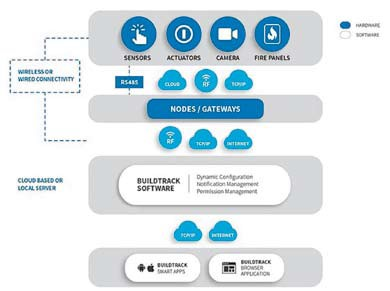
\includegraphics[width=0.8\textwidth]{image4}
  \caption{Стандартная архитектура системы пожарной безопасности на основе IoT}
\end{figure}

\begin{multicols}{2}

Системы оповещения и эвакуации граждан являются важной частью общей
системы пожарной безопасности. Они предназначены для предупреждения
людей о возможной опасности и организации эвакуации в случае пожара.
Существуют различные типы систем оповещения и эвакуации граждан, которые
могут быть использованы в зависимости от конкретной ситуации.

Одним из наиболее распространенных типов систем оповещения является
система громкоговорителей. Она включает в себя установку
громкоговорителей в зданиях и на улицах города, которые могут
воспроизводить звуковые сигналы для предупреждения людей о возможной
опасности. Некоторые системы громкоговорителей также могут
использоваться для оповещения людей о том, что они могут покинуть здание
в случае пожара.

Еще один тип системы оповещения -- это система SMS-уведомлений. Она
используется для отправки SMS-сообщений на мобильные телефоны людей,
которые зарегистрировали свои номера в системе. Такие системы могут быть
особенно полезны в крупных городах, где многие люди постоянно находятся
в движении.

Существуют также системы оповещения и эвакуации на основе световых
сигналов. Они могут использоваться в сочетании с системами
громкоговорителей или отдельно. Например, система оповещения на основе
световых сигналов может быть установлена в здании и использоваться для
предупреждения людей о пожаре, если в помещении слишком шумно для того,
чтобы использовать громкоговорители.

Кроме того, существуют также автоматические системы оповещения, которые
могут быть интегрированы с другими умными системами пожарной
безопасности. Например, система детектирования пожара на основе дыма
может быть интегрирована с системой оповещения для автоматического
предупреждения людей в здании о возможной опасности.

Все системы оповещения и эвакуации граждан имеют свои преимущества и
недостатки, которые могут зависеть от конкретных обстоятельств.

Далее приведены преимущества и недостатки некоторых распространенных
систем оповещения и эвакуации граждан:

Звуковая система оповещения и эвакуации. Это самый распространенный и
простой вид системы, который использует звуковой сигнал для оповещения и
направления людей на выход из здания.

Преимущества:

\begin{enumerate}
\def\labelenumi{\arabic{enumi}.}
\item
  Простота установки и использования;
\item
  Низкая стоимость.
\end{enumerate}

Недостатки:

\begin{enumerate}
\def\labelenumi{\arabic{enumi}.}
\item
  Неэффективность для людей со слабым слухом;
\item
  Ограниченность в передаче информации о характере и местоположении
  пожара.
\end{enumerate}

Система оповещения и эвакуации на основе световых сигналов. Эта система
использует световые сигналы, такие как мигающие огни, для оповещения и
направления людей к выходу из здания.

Преимущества:

\begin{enumerate}
\def\labelenumi{\arabic{enumi}.}
\item
  Эффективность для людей со слабым слухом;
\item
  Хорошая видимость в темноте.
\end{enumerate}

Недостатки:

\begin{enumerate}
\def\labelenumi{\arabic{enumi}.}
\item
  Ограниченность в передаче информации о характере и местоположении
  пожара;
\item
  Высокая стоимость.
\end{enumerate}

Система оповещения и эвакуации на основе текстовых сообщений. Эта
система использует текстовые сообщения, передаваемые через мобильные
устройства или другие коммуникационные каналы, для оповещения и
направления людей к выходу из здания.

Преимущества:

\begin{enumerate}
\def\labelenumi{\arabic{enumi}.}
\item
  Может обеспечить более точную информацию о характере и местоположении
  пожара;
\item
  Хорошая эффективность для людей со слабым зрением или слухом.
\end{enumerate}

Недостатки:

\begin{enumerate}
\def\labelenumi{\arabic{enumi}.}
\item
  Требуется наличие мобильных устройств или других коммуникационных
  средств;
\item
  Неэффективность, если люди не могут или не хотят получать текстовые
  сообщения.
\end{enumerate}

Система оповещения и эвакуации на основе виртуальной реальности является
инновационным подходом к созданию системы безопасности. Она использует
технологию виртуальной реальности, чтобы обучать людей, как действовать
в случае пожара или другой аварии, а также для эвакуации.

Преимущества:

\begin{enumerate}
\def\labelenumi{\arabic{enumi}.}
\item
  Увеличивает эффективность обучения и подготовки к чрезвычайным
  ситуациям, поскольку обучение проводится в условиях виртуальной
  реальности, которая более реалистична и захватывающа.
\item
  Увеличивает эффективность эвакуации, поскольку люди могут быть более
  знакомы с территорией и знать, куда следует направляться.
\item
  Уменьшает количество жертв в чрезвычайных ситуациях, поскольку люди
  будут лучше подготовлены и обучены действовать в таких ситуациях.
\end{enumerate}

Недостатки:

\begin{enumerate}
\def\labelenumi{\arabic{enumi}.}
\item
  Системы на основе виртуальной реальности могут быть дорогостоящими для
  создания и установки.
\item
  Система требует обновлений и технического обслуживания, чтобы
  гарантировать ее надежность и эффективность.
\item
  Некоторые люди могут испытывать дискомфорт или неудобства при
  использовании виртуальной реальности, что может отвлечь их от обучения
  или эвакуации.
\end{enumerate}

Системы оповещения и эвакуации на основе виртуальной реальности являются
новым направлением в развитии умных городов, поэтому пока что не
существует множества примеров реализации таких систем в реальных
городах.

Одним из примеров реализации подобной системы является проект,
воплощенный в жизнь компанией Luminous Group. Они разработали
виртуальную реальность, которая позволяет людям испытать пожарную
опасность, не находясь на самом объекте. Система состоит из нескольких
виртуальных тренажеров, которые имитируют ситуации пожаров различной
сложности. Посетитель может научиться пользоваться огнетушителями и
другими средствами пожаротушения, а также понять, как правильно и быстро
эвакуироваться из здания.

\begin{itemize}
\item
  Еще одним примером является проект, реализованный в городе Сингапур.
  Здесь была создана система AR-очков (очки дополненной реальности),
  которая позволяет людям быстро и безопасно покинуть здание в случае
  пожара. Система сканирует помещение и отображает на очках наиболее
  безопасный путь для эвакуации.
\item
  В России проекты по созданию систем оповещения и эвакуации на основе
  виртуальной реальности пока что не широко распространены, но многие
  компании работают в этом направлении, в том числе НИИ "Криста".
\end{itemize}

Система оповещения и эвакуации на основе световых сигналов является
одной из самых распространенных и простых систем в умных городах. Она
использует специальные световые сигналы, которые сигнализируют о
необходимости эвакуации или предупреждают об опасности. Примеры
реализации этой системы можно найти по всему миру.

\begin{itemize}
\item
  Например, в Японии система оповещения и эвакуации на основе световых
  сигналов используется во многих городах, включая Токио. Световые
  сигналы размещены во многих местах, в том числе на зданиях, мостах и
  автомобильных дорогах. Они могут быть использованы для предупреждения
  о землетрясениях, цунами и других природных катастрофах.
\item
  В США система оповещения и эвакуации на основе световых сигналов
  используется для предупреждения о торнадо. В некоторых городах
  установлены специальные световые сигналы, которые могут предупредить
  жителей о торнадо и указать направление, в котором необходимо
  двигаться для эвакуации.
\item
  В России система оповещения и эвакуации на основе световых сигналов
  также широко используется в умных городах. Например, в Москве и
  Санкт-Петербурге световые сигналы установлены на зданиях, мостах и
  других объектах, и используются для оповещения жителей о пожарах,
  авариях и других чрезвычайных ситуациях.
\end{itemize}

Однако, недостатком этой системы является то, что она может быть
ограничена в использовании в темное время суток или в условиях, когда
видимость снижена из-за дыма или тумана. Кроме того, световые сигналы
могут быть не заметны для людей с ограниченными возможностями зрения
(Рис. 5).

\end{multicols}

\begin{figure}[H]
  \centering
  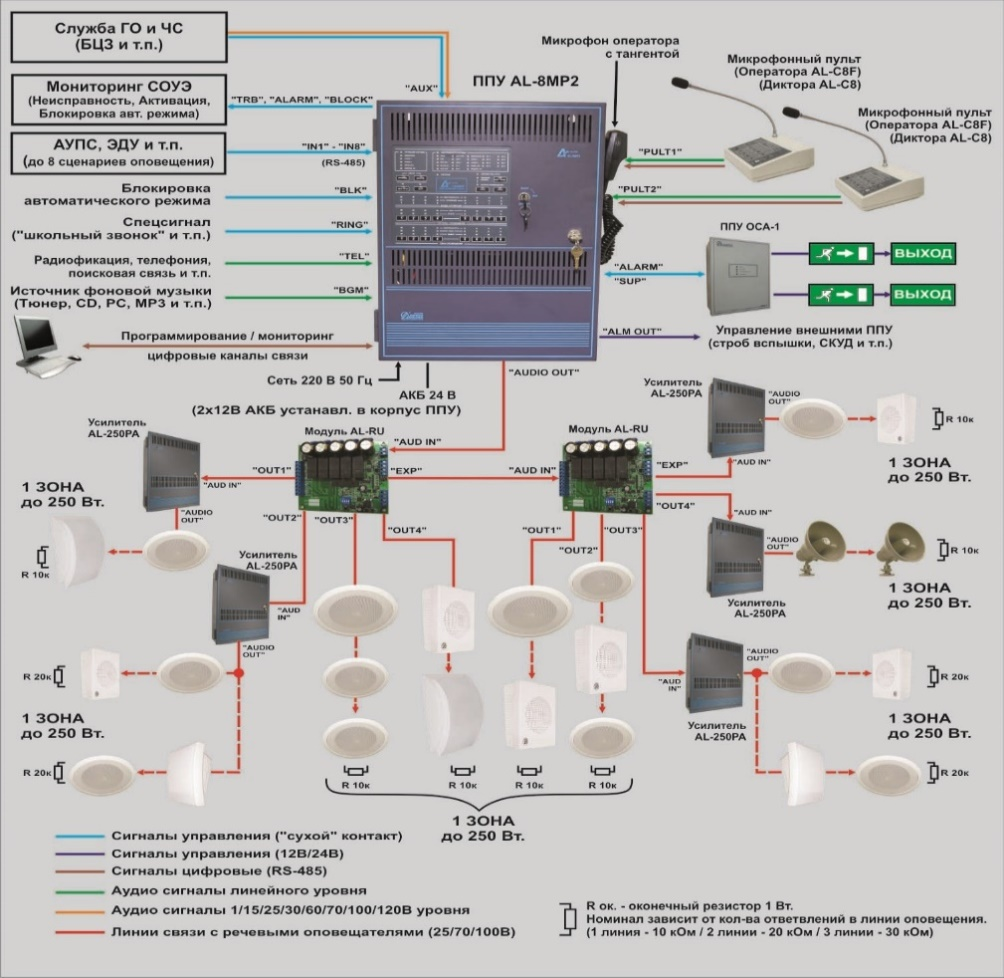
\includegraphics[width=0.8\textwidth]{image5}
  \caption{Система речевого оповещения о пожаре серии Альфа}
\end{figure}

\begin{multicols}{2}

Сравнение различных систем пожарной безопасности зависит от многих
факторов, включая тип здания, его назначение, размер и наличие
персонала. Ниже приведены общие характеристики и сравнение нескольких
типов систем пожарной безопасности.

Системы автоматического пожаротушения:

Преимущества: эффективность, автоматическое действие, надежность.

Недостатки: возможно повреждение имущества, высокая стоимость установки
и технического обслуживания.

Системы оповещения и эвакуации:

Преимущества: быстрое оповещение, возможность эвакуации, надежность.

Недостатки: требуют обучения и знания о процедурах эвакуации, могут
вызывать панику в людях, не способных на нормальное восприятие звуков.

Системы детектирования пожаров:

Преимущества: быстрое обнаружение пожара, возможность автоматической
активации других систем безопасности.

Недостатки: ложные срабатывания, высокая стоимость установки и
технического обслуживания.

Системы пассивной защиты от пожара:

Преимущества: надежность, эффективность, низкая стоимость.

Недостатки: не действуют на пожарном стадии, не способны обнаруживать
пожар.

Системы управления пожаром на основе IoT-технологий:

Преимущества: точность, быстрое обнаружение и управление пожаром,
удаленное управление, снижение вероятности ложных срабатываний.

Недостатки: высокая стоимость, сложность в установке и техническом
обслуживании.

Применимость разных систем пожарной безопасности может зависеть от
конкретных городских условий, таких как климат, наличие промышленных
зон, плотность населения и т.д. Например, в городах, где климат холодный
и снежный, система автоматического тушения пожаров водой может быть
менее эффективной из-за возможности замерзания воды и образования льда,
что затруднит доступ к возгоранию и усложнит работу пожарных.

С другой стороны, в городах с промышленными зонами, где может быть
большое количество горючих материалов и легко воспламеняемых веществ,
могут быть эффективны системы автоматического тушения пожаров, которые
используют специализированные химические вещества, такие как инертные
газы или порошок.

Также важным фактором может быть плотность населения и густота
застройки. В городах с большой плотностью населения и высокой застройкой
может быть трудно провести эвакуацию людей в случае пожара, поэтому
могут быть эффективны системы оповещения и эвакуации, которые используют
визуальные и звуковые сигналы, чтобы привлечь внимание граждан и
направить их на безопасный выход.

Таким образом, выбор системы пожарной безопасности должен основываться
на конкретных условиях города и требованиях к безопасности, а также на
эффективности, надежности и стоимости реализации и эксплуатации системы.

Умные технологии имеют огромный потенциал для улучшения систем пожарной
безопасности в умных городах. Многие инновации уже внедрены и успешно
работают, позволяя ускорить процессы обнаружения и тушения пожаров,
оповещения и эвакуации населения, а также минимизации ущерба от пожара
(Рис. 6).

Системы оповещения и эвакуации на основе IoT-технологий и виртуальной
реальности позволяют быстро обнаружить пожар и организовать эвакуацию,
даже если люди находятся внутри зданий, где не ощущают запах дыма или не
видят огонь. Автоматические системы пожаротушения на основе газа, пены,
порошка и воды позволяют быстро потушить пожар и предотвратить
распространение огня.

Системы мониторинга и детектирования пожаров, основанные на датчиках и
анализе больших данных, позволяют быстро обнаружить начальные стадии
пожара и принять меры для его тушения. Автоматические системы управления
пожаром на основе IoT-технологий позволяют быстро реагировать на пожар и
координировать действия пожарных бригад {[}10, 11{]}.

\end{multicols}

\begin{figure}[H]
  \centering
  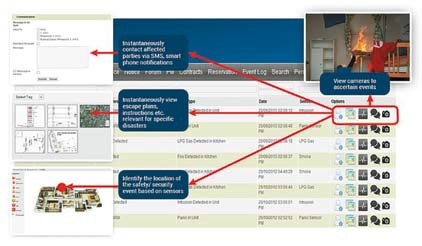
\includegraphics[width=0.8\textwidth]{image6}
  \caption{Пример централизованной системы контроля, позволяющей выявлять
чрезвычайные ситуации в пределах обширной территории}
\end{figure}

\begin{multicols}{2}

Каждая из систем имеет свои преимущества и недостатки, и выбор
конкретной системы должен основываться на характеристиках конкретного
города и его потребностях. Однако все они могут быть успешно
интегрированы в общую систему пожарной безопасности, что позволит
значительно повысить ее эффективность.

{\bfseries Выводы.} Умные системы пожарной безопасности имеют большой
потенциал для развития в будущем. С появлением новых технологий и
развитием искусственного интеллекта, умные системы пожарной безопасности
будут становиться все более эффективными и точными в предотвращении и
тушении пожаров. Одной из перспективных технологий является
использование беспилотных авиационных систем для наблюдения и тушения
пожаров, особенно там, где доступ человека затруднен или опасен. Также в
будущем умные системы пожарной безопасности могут быть установлены во
всех зданиях и сооружениях, и интегрированы с другими умными системами
города, такими как системы мониторинга качества воздуха, системы
управления транспортом и энергетические сети. Другой перспективной
технологией является использование блокчейн-технологии для создания
безопасных и надежных систем пожарной безопасности. Блокчейн может
обеспечить децентрализованное хранение данных о системах пожарной
безопасности и связанных с ними рисках, что может помочь в
предотвращении пожаров и быстрой реакции на них.

В целом, умные технологии имеют огромный потенциал для улучшения систем
пожарной безопасности в умных городах, что может привести к снижению
рисков и сохранению жизней.
\end{multicols}

\emph{Работа выполнена за счет средств грантового финансирования научных
исследований на 2023-2025 годы по проекту ИРН АР19678157.}

{\bfseries Литература}

1. Ву Т.З. Анализ систем автоматизированного управления умным домом //
Молодой ученый, 2011. -- №4. Т.1. -- С. 28-29. (in Eng).

2. А.Ф. Котюк. Датчики в современных измерениях. -- М.: «Радио и связь»,
2006. -- 96 с. (in Russ).

3. Дж. Фрайден. Современные датчики. -- М.: «Техносфера», 2005. -- 592
с. (in Russ).

4. Е.А. Тесля. «Умный дом» своими руками. Строим интеллектуальную
цифровую систему в своей квартире / Тесля Е.А. -- СПб., 2008. -- 224 с.
(in Russ).

5. Intelligent Buildings: Design, Management \& Operation / edited by
Derek Clements-Croome. -- London: Thomas Telford Publishing, 2004. --
408 p. (in Eng).

6. Г.З. Зиятбекова, А.Т. Мазакова, А.Д. Бургегулов, Е.Б. Муратов.
Разработка энергосберегающей системы «Умный офис» и его принципы работы
// Вестник КазУТБ. -- Нур-Султан, 2022. -- № 1(14). -- С. 13-18. (in
Russ).

7. Ч. Платт. Электроника: логические микросхемы, усилители и датчики для
начинающих. -- СПб.: БХВ-Петербург, 2015. -- 448 с. (in Eng).

8. Т. Рашид. Создаем нейронную сеть. -- СПб.: ООО «Альфа-книга», 2018.
-- 272 с. (in Russ).

9. К.Е. Климентьев. Системы реального времени. -- Самара: Самар.гос.
аэрокосм. ун-т, 2008. -- 45 с. (in Russ).

10. Р. Каллан. Нейронные сети. Краткий справочник -- М.: ООО «И.Д.
Вильямс», 2017. -- 288 с. (in Russ).

11. С.В. Аксенов, В.Б. Новосельцев. Организация и использование
нейронных сетей (методы и технологии). -- Томск: Изд-во НТЛ, 2006. --
128 с. (in Russ).

{\bfseries\centering References}

1. Wu T.Z. Analysis of automated control systems for smart house //
Young Scientist, 2011. -- No. 4. -- VOL. 1. -- Pр. 28-29. (in Eng)

2. A.F. Kotyuk. Sensors in Modern Measurements. -- M.: Radio and
Communications, 2006. -- 96 p. (in Russ)

3. J. Fryden. Modern Sensors. -- M.: Technosphere, 2005. -- 592 p. (in
Russ)

4. E.A. Tesla. "Smart House with my own hands. Building an intelligent
digital system in your apartment / Teslya E.A. -- SPb., 2008. -- 224 p.
(in Russ)

5. Intelligent Buildings: Design, Management \& Operation / edited by
Derek Clements-Croome. -- London: Thomas Telford Publishing, 2004. --
408 p. (in Eng)

6. G.Z. Ziyatbekova, A.T. Mazakova, A.D. Burgegulov, E.B. Muratov.
Development of energy-saving system "Smart Office" and its operating
principles // Bulletin of KazUTB. -- Nur-Sultan, 2022. -- No. 1(14). --
Pp. 13-18. (in Russ)

7. Ch. Platt. Electronics: Logic Circuits, Amplifiers and Sensors for
Beginners. -- SPb: BHV-Peterburg, 2015. -- 448 p. (in Eng)

8. Т. Rashid. Creating a neural network. -- St. Petersburg: OOO
"Alpha-book", 2018. -- 272 p. (in Russ)

9. K.E. Klimentiev. Real-time systems. -- Samara: Samara State Aerospace
University, 2008. -- 45 p. (in Russ)

10. Р. Callan. Neural networks. A Quick Reference Guide. -- M.: I.D.
Williams LLC, 2017. -- 288 p. (in Russ)

11. S.V. Aksenov, V.B. Novoseltsev. Organization and use of neural
networks (methods and technologies). -- Tomsk: NTL Publisher, 2006. --
128 p. (in Russ)

\emph{{\bfseries Сведения об авторах}}

Бургегулов А. Д. -- докторант КазНУ имени аль-Фараби, Алматы, Казахстан,
\href{mailto:dizel_kz@bk.ru}{\nolinkurl{dizel\_kz@bk.ru}}

Мазаков Т.Ж. -- доктор физико-математических наук, главный научный
сотрудник Института Информационных и вычислительных технологий КН МНВО
РК, профессор НАО Казахского национального университета имени
аль-Фараби, Алматы, Казахстан,
\href{mailto:tmazakov@mail.ru}{\nolinkurl{tmazakov@mail.ru}}

Зиятбекова Г.З. -- PhD, и.о. доцента НАО Казахского национального
университета имени аль-Фараби; старший научный сотрудник Института
Информационных и вычислительных технологий КН МНВО РК, Алматы,
Казахстан,
\href{mailto:ziyatbekova@mail.ru}{\nolinkurl{ziyatbekova@mail.ru}}

Саметова А.А. -- докторант КазНУ имени аль-Фараби, Алматы, Казахстан,
sametova\_aygerim\href{mailto:amirkhanov.b@gmail.com}{@mail.}ru

Джолдасова Б.У. -- магистрант КазНУ имени аль-Фараби, Алматы, Казахстан,
bagilaurel@gmail.com

\emph{{\bfseries Information about authors}}

Burgegulov A. D. -- doctoral student at Al-Farabi Kazakh National
University, Almaty, Kazakhstan, dizel\_kz@bk.ru

Mazakov T. Zh. -- NAO Al-Farabi Kazakh National University, doctor of
physical and mathematical sciences, professor, Almaty, Kazakhstan, Chief
Researcher at the RSE Institute of Information and Computational
Technologies of the National Academy of Sciences of the Republic of
Kazakhstan, Almaty, Kazakhstan,
\href{mailto:tmazakov@mail.ru}{\nolinkurl{tmazakov@mail.ru}}

Ziyatbekova G. Z. -- PhD, Acting Associate Professor NAO Al-Farabi
Kazakh National University; Senior Researcher at the RSE Institute of
Information and Computational Technologies of the National Academy of
Sciences of the Republic of Kazakhstan, Almaty, Kazakhstan,
ziyatbekova@mail.ru

Sametova Aigerim Aidarkyzy -- doctoral student at Al-Farabi Kazakh
National University, Almaty, Kazakhstan,
sametova\_aygerim\href{mailto:amirkhanov.b@gmail.com}{@mail.}ru

Joldassova Bagila Ummetovna -- graduate student at Al-Farabi Kazakh
National University, Almaty, Kazakhstan, bagilaurel@gmail.com
